\chapter{\textcolor{blue}{Posturas ou poses do corpo}}\index{Postura}\index{Pose}


Para a explicação das posturas, neste capítulo, serão usados dois tipos diferentes de vista de câmera;
uma vista é frontal à pessoa, 
que representa a visão desde o ponto de vista do par de dança colocado ao frente do executante do movimento; 
e outra câmera com vista lateral, 
que representa a vista de um observador externo situado ao lado direito do executante do movimento; 
conforme o descrito na Figura \ref{fig:vistacamera}.
Em todas as figuras está colorida a perna esquerda com a cor cinza, e a perna direita com um cor preto;
o triangulo $\triangle$ indica o pé que contem o peso do corpo.
\begin{figure}[h]
  \centering
    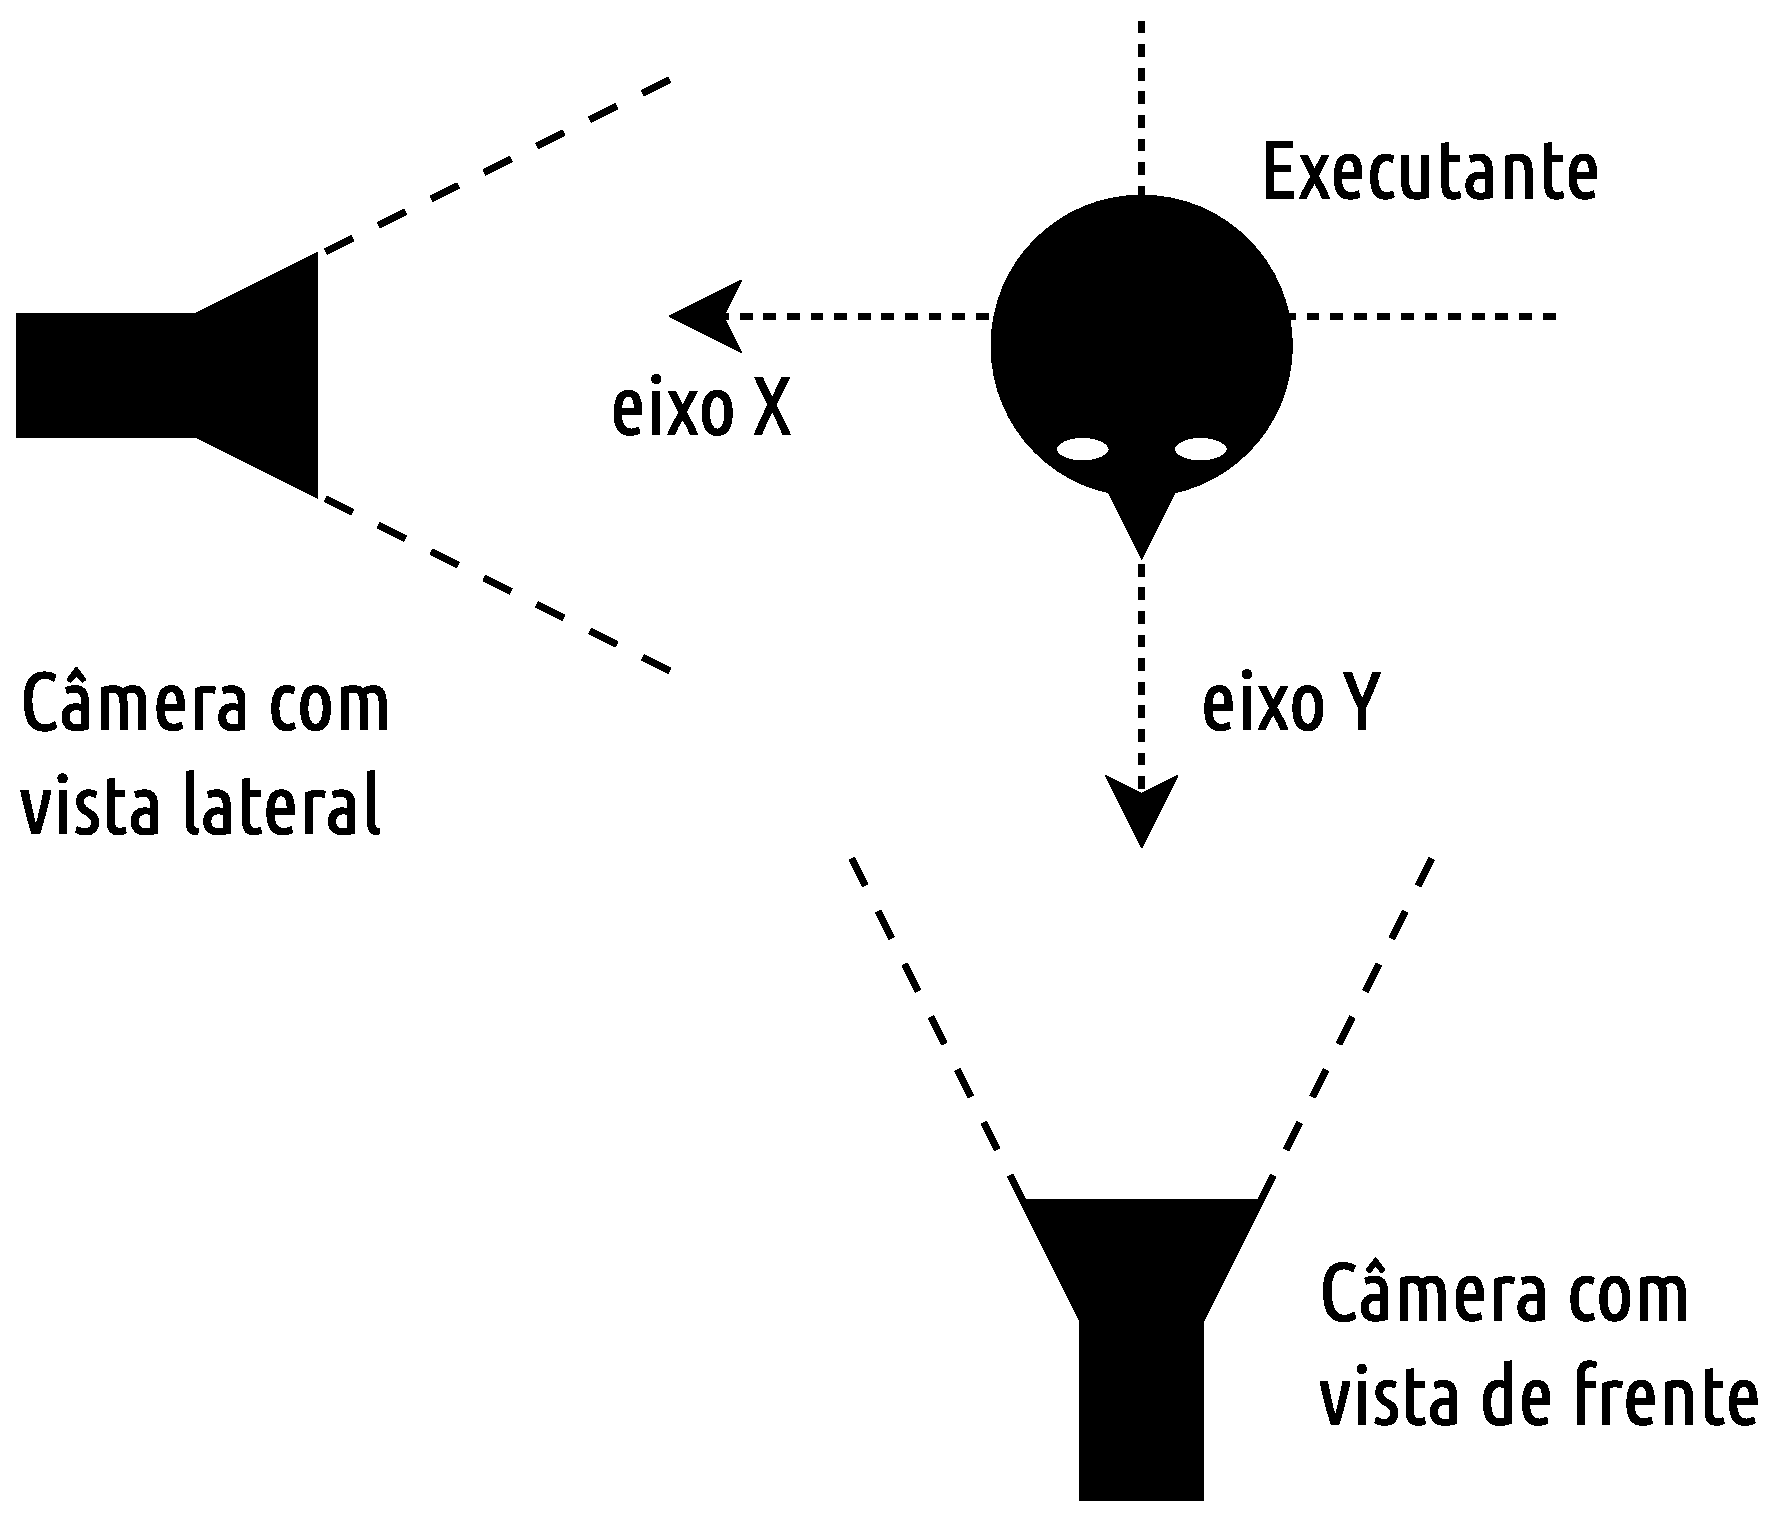
\includegraphics[width=0.5\textwidth]{chapters/cap-posturas/vistas.eps}
  \caption{Descrição da posição das câmeras nas vistas usadas nas imagens mostradas neste capítulo.}
  \label{fig:vistacamera}
\end{figure}


%%%%%%%%%%%%%%%%%%%%%%%%%%%%%%%%%%%%%%%%%%%%%%%%%%%%%%%%%%%%%%%%%%%%%%%%%%%%%%%%
%%%%%%%%%%%%%%%%%%%%%%%%%%%%%%%%%%%%%%%%%%%%%%%%%%%%%%%%%%%%%%%%%%%%%%%%%%%%%%%%
\section{\textcolor{blue}{Posturas pessoais}}



\subsection{\textcolor{blue}{ Posturas de Frente }}

A postura \text{frente-direita} é uma postura a frente com peso do corpo na perna direita, ver Figura \ref{fig:frentedireita}.
A postura \text{frente-esquerda} é uma postura a frente com peso do corpo na perna esquerda, ver Figura \ref{fig:frenteesquerda}.
\begin{figure}[H]
    \centering
    \begin{subfigure}[b]{0.3\textwidth}
        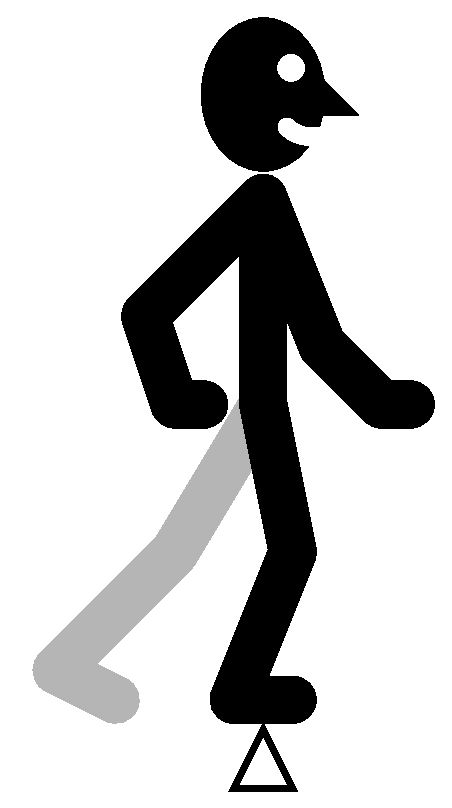
\includegraphics[height=4cm]{chapters/cap-posturas/postura-ft-frente-der.eps}
        \caption{Postura frente-direita}
        \label{fig:frentedireita}
    \end{subfigure}
    ~ %add desired spacing between images, e. g. ~, \quad, \qquad, \hfill etc. 
      %(or a blank line to force the subfigure onto a new line)
    \begin{subfigure}[b]{0.3\textwidth}
        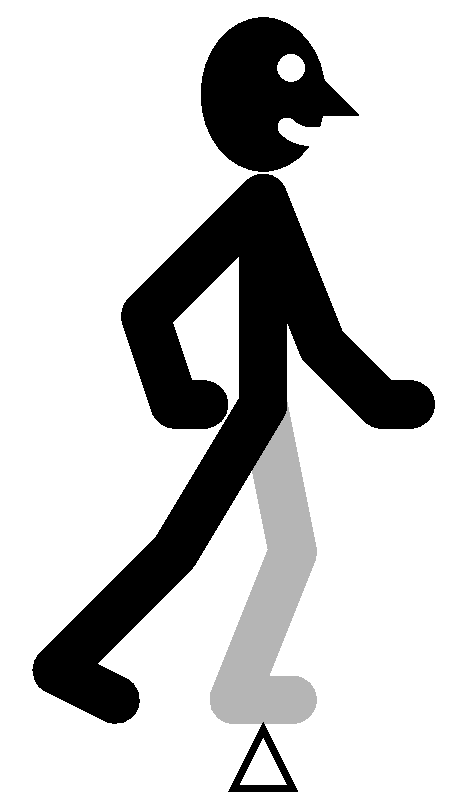
\includegraphics[height=4cm]{chapters/cap-posturas/postura-ft-frente-esq.eps}
        \caption{Postura frente-esquerda}
        \label{fig:frenteesquerda}
    \end{subfigure}
    \caption{Posturas a frente  com vista lateral}\label{fig:frentederesq}
\end{figure}

Exemplos: Frente-trás, escovinhas para frente, etc


\subsection{\textcolor{blue}{ Posturas de  trás}}


A postura \text{trás-direita} é uma postura a trás com peso do corpo na perna direita, ver Figura \ref{fig:trasdireita}.
A postura \text{trás-esquerda} é uma postura a trás com peso do corpo na perna esquerda, ver Figura \ref{fig:trasesquerda}.
\begin{figure}[H]
    \centering
    \begin{subfigure}[b]{0.3\textwidth}
        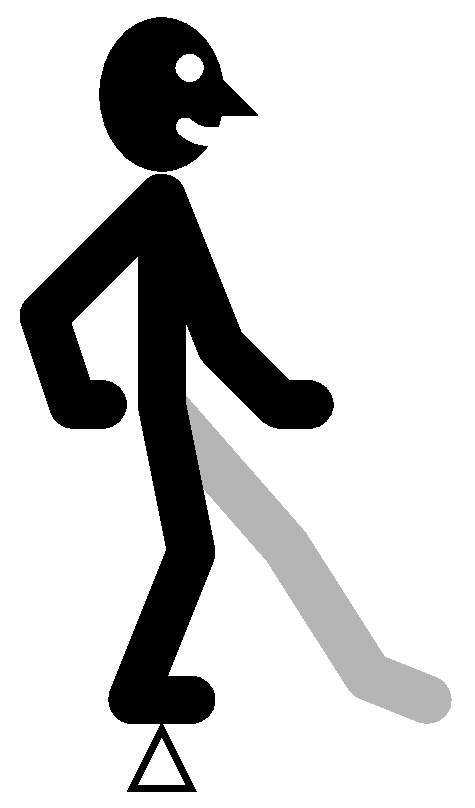
\includegraphics[height=4cm]{chapters/cap-posturas/postura-ft-tras-der.eps}
        \caption{Postura trás-direita}
        \label{fig:trasdireita}
    \end{subfigure}
    ~ %add desired spacing between images, e. g. ~, \quad, \qquad, \hfill etc. 
      %(or a blank line to force the subfigure onto a new line)
    \begin{subfigure}[b]{0.3\textwidth}
        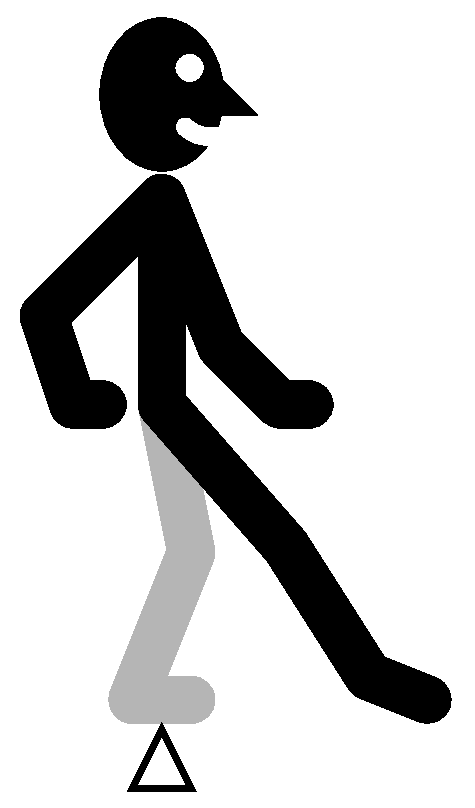
\includegraphics[height=4cm]{chapters/cap-posturas/postura-ft-tras-esq.eps}
        \caption{Postura trás-esquerda}
        \label{fig:trasesquerda}
    \end{subfigure}
    \caption{Posturas a trás  com vista lateral}\label{fig:trasderesq}
\end{figure}

Exemplo: Frente-trás, escovinhas para atras, etc

\subsection{\textcolor{blue}{ Posturas ao Lado}}

A postura \text{lado-direita} é uma postura ao lado com peso do corpo na perna direita, ver Figura \ref{fig:ladodireita}.
A postura \text{lado-esquerda} é uma postura ao lado com peso do corpo na perna esquerda, ver Figura \ref{fig:ladoesquerda}.
\begin{figure}[H]
    \centering
    \begin{subfigure}[b]{0.3\textwidth}
        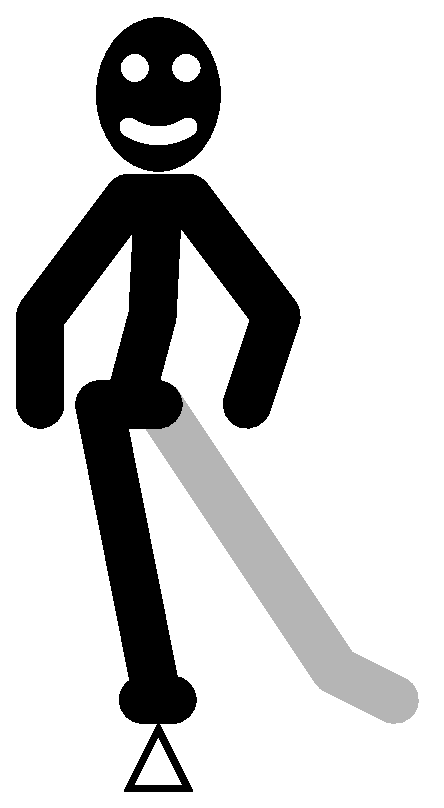
\includegraphics[height=4cm]{chapters/cap-posturas/postura-lateral-der.eps}
        \caption{Postura lado-direita}
        \label{fig:ladodireita}
    \end{subfigure}
    ~ %add desired spacing between images, e. g. ~, \quad, \qquad, \hfill etc. 
      %(or a blank line to force the subfigure onto a new line)
    \begin{subfigure}[b]{0.3\textwidth}
        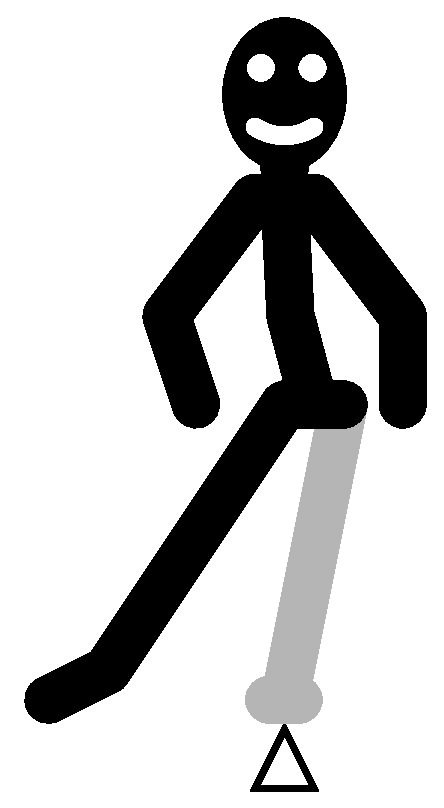
\includegraphics[height=4cm]{chapters/cap-posturas/postura-lateral-esq.eps}
        \caption{Postura lado-esquerda}
        \label{fig:ladoesquerda}
    \end{subfigure}
    \caption{Posturas ao lado  com vista de frente}\label{fig:ladoderesq}
\end{figure}


Exemplo: balanço.

\subsection{\textcolor{blue}{ Posturas de Cruzadas }}
Exemplo: cruzado

\subsection{\textcolor{blue}{ Posturas de facão dividido}}
Ou simplesmente chamado postura de facão
Exemplo: Facão, pião finalizando em facão

\subsection{\textcolor{blue}{ Posturas de facão invertido}}

Exemplo: escovinha desde facão invertido.


%%%%%%%%%%%%%%%%%%%%%%%%%%%%%%%%%%%%%%%%%%%%%%%%%%%%%%%%%%%%%%%%%%%%%%%%%%%%%%%%
%%%%%%%%%%%%%%%%%%%%%%%%%%%%%%%%%%%%%%%%%%%%%%%%%%%%%%%%%%%%%%%%%%%%%%%%%%%%%%%%
\section{\textcolor{blue}{Posturas do casal}}

\begin{itemize}
\item Cruzado invertido (ex: caminhada de casal).
\item X (ex: caminhada, romario).
\end{itemize}
